\chapter{Theoretical framework}
\label{ch:theory}

This chapter gives an outline of the theoretical concepts and models used in this thesis. It is split into two parts: First, the Standard Model of elementary particle physics is discussed, with a heavy emphasis on the top quark. Secondly, several hypothesized extensions of the Standard Model, relevant for the searches presented in ??, are briefly introduced and compared.

\section{Standard Model}

% content:
% particles, interactions, alphaEW, alphas
% top quark: mass, width, lifetime; decay into Wb;
% Yukawa coupling to Higgs, spin analyzing power
% Higgs mechanism: Higgs doublet in the SM, symmetry breaking, result: massive scalar particle; mass, coupling to massive particles
% pp -> ttbar: production diagrams (tree level), production modes (gg / qq), decays: allhad, semilep, dilep; mtt spectrum (?); spin states of ttbar
% spin density matrix: decomposition into polarizations and correlations, linear observables; cite new measurements
% nonperturbative: resummations close to the threshold, Couloumb resummation --> sorta bound state; comparison with J/Psi and Upsilon (large top width), difficulty of modeling: singlet v octet, Fuks model: singlet only, effective model, hints for observation in entanglement paper

The Standard Model of elementary particle physics, often simply called the Standard Model or SM, is, at the time of writing, the most successful theory describing the fundamental particles making up our universe. It is the result of a steady progression of increasingly complex models, starting with the introduction of quantum mechanics in the early 20th century and ending - for now - with the discovery of the Higgs boson at the LHC in 2012. The model has been extensively tested at many different experiments, most importantly the large collider experiments like LEP, the Tevatron, and the LHC. So far, it has survived all these tests with excellence.

\begin{figure}[ht]
    \centering
    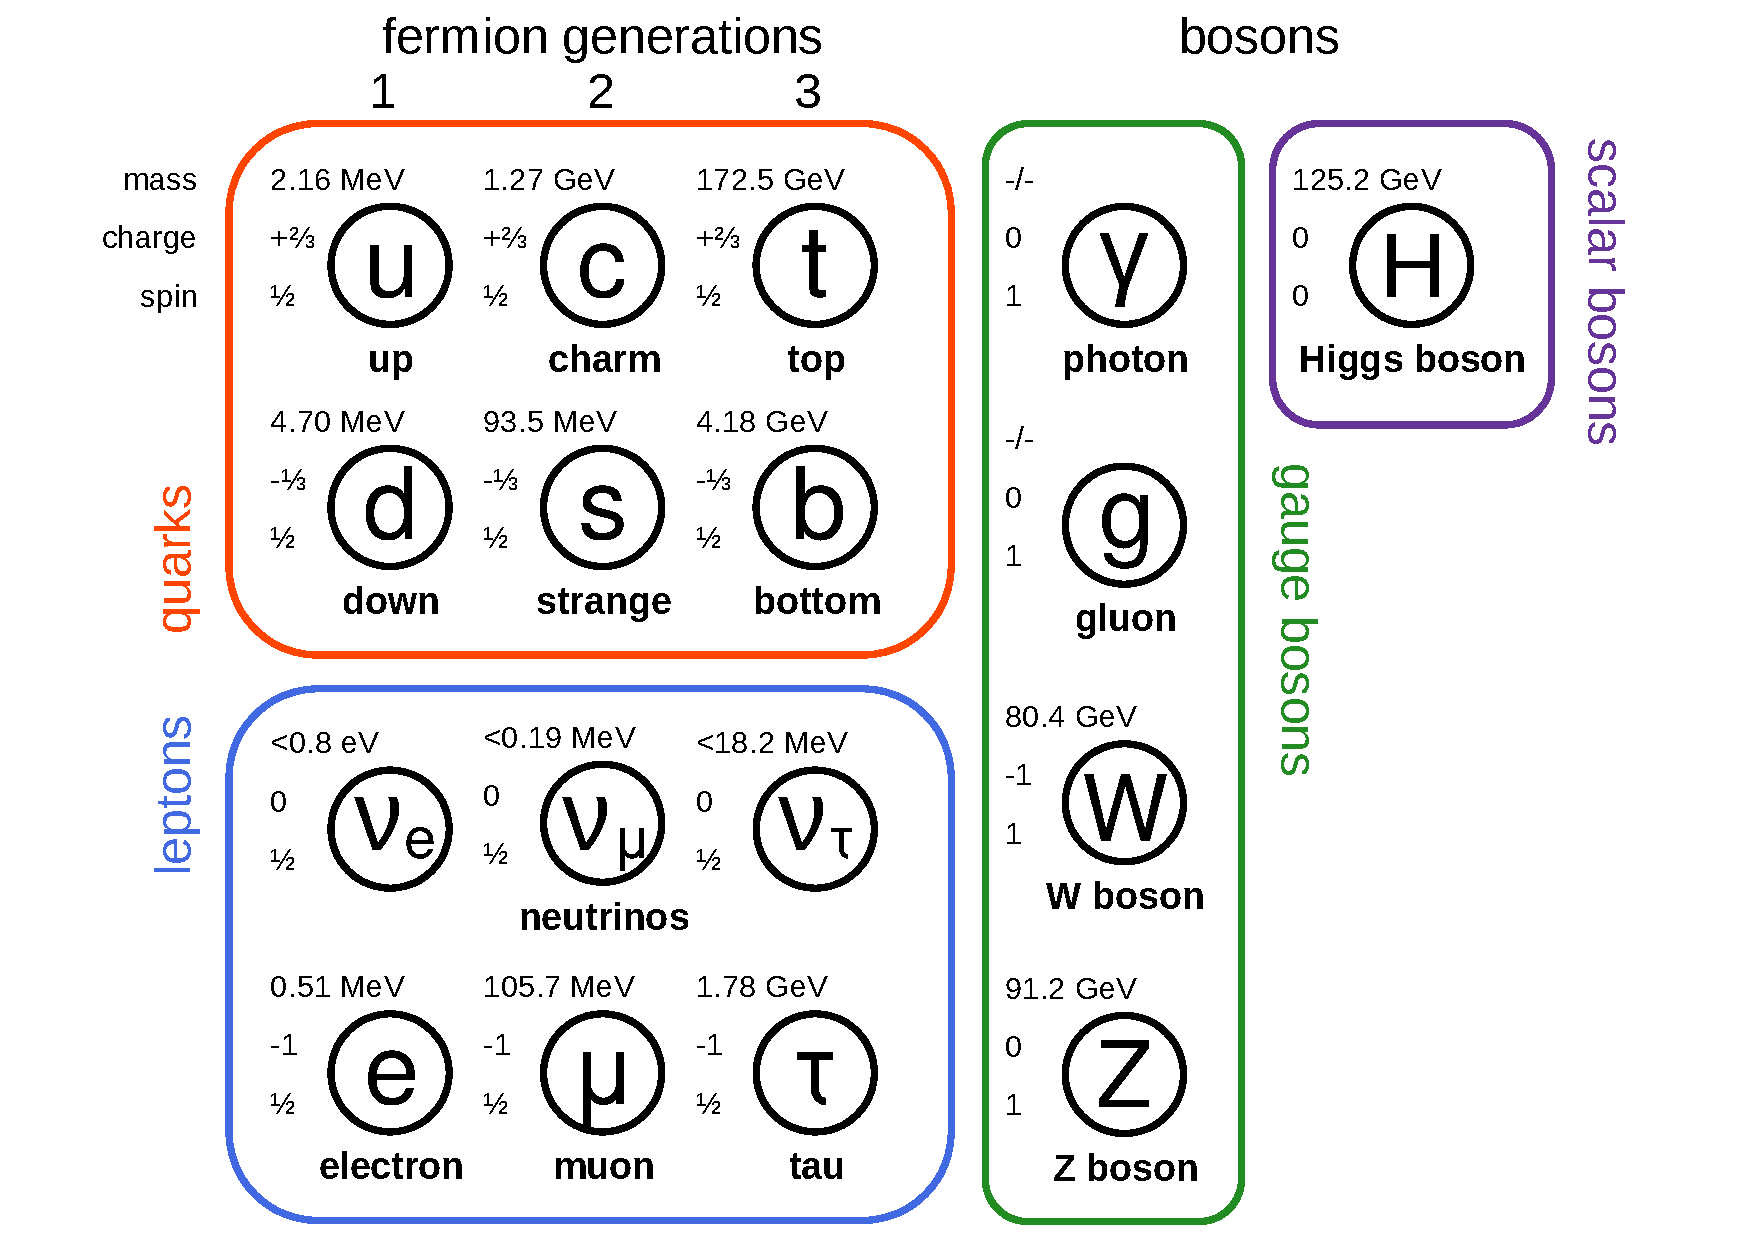
\includegraphics[width=0.9 \textwidth]{figures/smsketch_colors.pdf}
    \caption{Schematic depiction of the particle content of the Standard Model, showing the seventeen fundamental particles, split into six quarks, six leptons, four gauge bosons, and the Higgs boson. The masses, electromagnetic charges, and spin of the particles is given next to the labels. Mass information is taken from \citere{PDG:2022pth}.}
    \label{fig:theory:sm}
\end{figure}

The SM is formulated as a relativistic quantum field theory (QFT). That is, its most fundamental objects are fields acting on four-dimensional spacetime which, after a quantization procedure, yield physically observable particles as fundamental excitations. By the usual counting scheme, there exist seventeen different such fields, which can be classified into different groups. The first group consists of the twelve fermions, which have spin $\frac{1}{2}$ and make up all visible matter. They are further split into the leptons, consisting of three electrically charged leptons - electron, muon, and tau lepton - and three corresponding electrically neutral neutrinos, as well as the quarks, of which there are six different flavors, called up, down, strange, charm, bottom, and top. The quarks have fractional electric charge, and in addition carry color charge as their defining property. Of note is that the fermions are also split into three generations, with each generation consisting of a charged lepton, a neutrino, and two quarks. The only fundamental differences between the particles of different generations are their masses, though the resulting physically observable properties, such as the lifetime, might be dramatically different.

The second group of particles are the bosons, which have integer spin. Here, the four gauge bosons with spin 1 act as the force carriers of the four fundamental interactions described by the SM: the photon, for the electromagnetic interaction with coupling strength $\alpha_{\mathrm{elm}}$; the W and Z bosons, for the weak interaction with coupling strength $\alpha_W$; and the gluon, for the strong interaction with coupling strength $\alpha_S$. At high enough energies, the electromagnetic and weak interaction unify into the electroweak interaction (coupling strength $\alpha_{\mathrm{EW}}$). The last and final particle is the Higgs boson, which has spin 0. Its most important role in the SM is to give mass to the fermions, as well as the W and Z bosons, through the so-called Higgs mechanism, which is briefly outlined in ??.

\subsection{Top quark}

All results presented as part of this thesis focus on one particular fundamental particle: the top quark. As such, it will be described in further detail in this section.

The top quark was first discovered in ?? at the Tevatron by the CDF and D0 experiments (refs). With a rest mass of $m_t = \SI{172.5}{\GeV}$, the top quark is the most massive known fundamental particle, and as a result it has unique properties compared to the other quarks: Its extremely short lifetime of $\approx \SI{5e25}{\s}$ is lower than the typical time needed for a quark to hadronize under the strong interaction, making it the only bare quark - that is, the only quark which,  via its decay products, is observable outside of hadrons. Among others, a consequence of this is that it fully preserves spin information during its decay, while such information is typically lost for other quarks during hadronization. More details on this are found in \cref{sec:theory:spindensity}.

A second extraordinary property of the top quark that follows from its high mass is its large Yukawa coupling to the SM Higgs boson, which is of order one. As a result, the Higgs boson couples preferentially to the top quark of all SM particles, and the study of both the SM Higgs boson and hypothetical additional Higgs bosons (see \cref{sec:theory:bsm}) is tightly connected to the top quark. 

In the SM, the top quark decays to a bottom quark and a W boson with a branching ratio (BR) of almost 100\% (to the degree that all other decays are commonly neglected). The W boson, in turn, can decay either to a charged lepton (e, $\mu$ or $\tau$) and the corresponding neutrino with a BR of $\sim 32.6\%$, or to a pair of quarks (one up- and one down-type) with a BR of $\sim 67.4\%$. This results in different final states for top production processes, which are discussed more in \cref{sec:theory:ttbar}.

\subsection{Higgs mechanism}

The Higgs boson is the most recently discovered particle of the SM. Its existence was confirmed in 2012 at the LHC by the ATLAS and CMS collaborations (refs), firmly establishing the SM in its current form as the accepted description of elementary particle physics. While this work does not focus on the SM Higgs boson as it does on the top quark, a short discussion of its role in the SM - the so-called Higgs mechanism - is relevant for possible SM extensions to additional Higgs bosons, which are searched for in \cref{ch:ah,ch:alps}.

In the SM Lagrangian, the Higgs boson appears as a complex doublet $\phi$ in the form

\begin{equation}
    \mathcal{L}_{\mathrm{SM}} \subset \left(D_\mu \phi\right)^\dagger D^\mu \phi + V(\phi)
\end{equation}

\noindent where $D_\mu$ is the covariant derivative, containing the minimal coupling to the gauge fields, and the Higgs potential $V(\phi)$ is 

\begin{equation}
    V(\phi) = \mu^2 \phi^\dagger \phi - \lambda (\phi^\dagger \phi)^2 .
\end{equation}

Here, $\mu^2$ and $\lambda$ are free parameters of the model. If both parameters are positive, this potential (known as the "Mexican hat potential") has a minimum at a non-zero value of

\begin{equation}
    | \phi | = \frac{\mu}{\sqrt{2 \lambda}} \equiv \frac{v}{\sqrt{2}}
\end{equation}

\noindent with the vacuum expectation value $v = \mu / \sqrt{\lambda}$. On the other hand, the minimum - corresponding to the vacuum state - is degenerate with respect to the three phases (i.e. the $SU(2)$ symmetry) of the complex doublet.

In the Higgs mechanism, this symmetry is now spontaneously broken in the transition from the high-energy state of the early universe (where the minimum is at $|\phi| = 0$) to the low-energy state observed today. The physical particles after symmetry breaking are then described by fluctuations around the new vaccum state. If the Higgs field were to be considered on its own, this would lead to one massive (corresponding to fluctuations in the $|\phi|$ direction) and three massless degrees of freedom (corresponding to the phases).

However, the interaction with the electroweak gauge fields encoded within $D_\mu$ leads to the massless degrees of freedom being absorbed into the gauge fields (ref). This turns three of the four massless spin-1 gauge fields of the electroweak Lagrangian (with two degrees of freedom each) into massive fields instead (which have an additional longitudinal polarization, and thus three degrees of freedom). These three massive gauge fields are identified with the W and Z bosons, while the remaining massless field is identified with the photon. Finally, the leftover massive degree of freedom from the Higgs doublet $\phi$ is identified with the spin-0 boson observed at the LHC.

The resulting masses of the Z, W and Higgs bosons can be predicted as a function of $\mu^2$, $\lambda$ and the electroweak couplings and thus used to test the Higgs mechanism. In addition to the electroweak bosons, the Higgs mechanism can also give masses to fermions (charged leptons and quarks) by including a Yukawa interaction term in the Lagrangian. This results in couplings between the SM Higgs boson and the different fermions that are proportional to the respective fermion mass, leading to the largest coupling to the top quark. In possible extensions of the SM, this proportionality might be modified, making Yukawa coupling measurements attractive as tests of the SM.

\section{The \pptt process}
\label{sec:theory:ttbar}

In proton-proton collisions at the LHC, the dominant production mode of top quarks is the production of a top-antitop quark pair (\ttbar). The different parts of this thesis all focus on this process in different ways, and so this chapter gives a detailed overview of relevant effects.

At LO in QCD, there are three diagrams (up to permutations of initial and final states) contributing to \ttbar production, which can be seen in \cref{fig:theory:ttbar}. They differ in their initial states: the first two diagrams are induced by gluon fusion, while the last one is induced by quark fusion (mostly from $\mathrm{u \bar{u}}$ and $\mathrm{d \bar{d}}$). The fraction of these is determined by the corresponding parton densities; at a center-of-mass energy of $\sqrt{s} \geq \SI{13}{\TeV}$, gluon fusion dominates with a fraction of roughly 90\%.

\begin{figure}[t]
    \centering
    \begin{tikzpicture}[baseline=(current bounding box.center)]
      \begin{feynman}
        \vertex (i1) {\(g\)};
        \vertex [below=2.0 cm of i1] (i2) {\(g\)};
        \vertex [right=1.5 cm of i1] (a);
        \vertex [right=1.5 cm of i2] (b);
        \vertex [right=1.5 cm of a] (f1) {\(t\)};
        \vertex [right=1.5 cm of b] (f2) {\(\bar{t}\)};
        \diagram* {
          (i1) -- [gluon] (a),
          (i2) -- [gluon] (b),
          (f1) -- [anti fermion] (a) -- [anti fermion, edge label'=\(t\)] (b) -- [anti fermion] (f2)
        };
      \end{feynman}
    \end{tikzpicture}
    \hfill
    \begin{tikzpicture}[baseline=(current bounding box.center)]
      \begin{feynman}
        \vertex (a) ;
        \vertex [above left=1.3 cm of a] (i1) {\(g\)};
        \vertex [below left=1.3 cm of a] (i2) {\(g\)};
        \vertex [right=1.5 cm of a] (b);
        \vertex [above right=1.3 cm of b] (f1) {\(t\)};
        \vertex [below right=1.3 cm of b] (f2) {\(\bar{t}\)};
        \diagram* {
          (i1) -- [gluon] (a) -- [gluon] (i2),
          (a) -- [gluon, edge label'=\(g\)] (b),
          (f1) -- [anti fermion] (b) -- [anti fermion] (f2)
        };
      \end{feynman}
    \end{tikzpicture}
    \hfill
    \begin{tikzpicture}[baseline=(current bounding box.center)]
      \begin{feynman}
        \vertex (a) ;
        \vertex [above left=1.3 cm of a] (i1) {\(q\)};
        \vertex [below left=1.3 cm of a] (i2) {\(\bar{q}\)};
        \vertex [right=1.5 cm of a] (b);
        \vertex [above right=1.3 cm of b] (f1) {\(t\)};
        \vertex [below right=1.3 cm of b] (f2) {\(\bar{t}\)};
        \diagram* {
          (i1) -- [fermion] (a) -- [fermion] (i2),
          (a) -- [gluon, edge label'=\(g\)] (b),
          (f1) -- [anti fermion] (b) -- [anti fermion] (f2)
        };
      \end{feynman}
    \end{tikzpicture}
    \caption{\textbf{Feynman diagrams for \pptt.} The three diagrams (up to permutations) that contribute to the \pptt process at LO in QCD.}
    \label{fig:theory:ttbar}
\end{figure}

\subsection{Spin density matrix}
\label{sec:theory:spindensity}

\subsection{Non-perturbative effects}

\section{Beyond the Standard Model}
\label{sec:theory:bsm}

\subsection{Extended Higgs sector models}
\label{sec:theory:hext}

\subsection{Axion-Like Particles}

\chapter{Monte Carlo event generation}

\section{Monte Carlo method}

\section{Matrix Element generators}

\section{Parton showers and matching}
